\documentclass{beamer}
\usepackage{../tut-slides}
\usepackage{../mathoperatorsAuD}

\usepackage{lmodern}
\usepackage{amsmath,amssymb}
\usepackage{stmaryrd}
\usepackage{enumerate}
%\usepackage[inline]{enumitem} 		%customize label
%\newcommand{\labelitemi}{\raisebox{1pt}{\scalebox{.9}{$\blacktriangleright$}}}
%\newcommand{\labelitemii}{$\vartriangleright$}
%\newcommand{\labelitemiii}{--}
\setbeamertemplate{itemize item}{\raisebox{1pt}{\scalebox{.9}{$\blacktriangleright$}}}
\setbeamertemplate{itemize subitem}{$\vartriangleright$}

\usepackage{booktabs}
\usepackage{tabularx}
\usepackage{tabu}
\newcommand*\head{\rowfont{\bfseries}}
\newcommand*{\tw}{\rowfont{\ttfamily}}
\renewcommand{\tabularxcolumn}[1]{>{\hspace{0pt}}m{#1}}
\usepackage{multirow}

\usepackage{cancel}

\usepackage{empheq}
\newcommand*\widefbox[1]{\fbox{\hspace{2em} #1 \hspace{2em}}}

\usepackage{tcolorbox}
\newtcolorbox{mymathbox}[1][]{colback=white, sharp corners, #1}

\usepackage{xcolor}
\usepackage{listings}
\newcommand*{\ttfamilywithbold}{\fontfamily{lmtt}\selectfont}
\lstset{numbers=left, 
	numberstyle=\tiny, 
	breaklines=true,
	backgroundcolor=\color{cdgray!10},
	numbersep=5pt,
	language=C,
	tabsize=2,
	basicstyle=\ttfamilywithbold,
	showstringspaces=false} 
\lstdefinestyle{example}{
	basicstyle=\footnotesize\ttfamilywithbold,   
	breakatwhitespace=false,         % sets if automatic breaks should only happen at whitespace
	breaklines=true,                 % sets automatic line breaking
	commentstyle=\itshape,    	     % comment style
	escapeinside={\%*}{*)},          % if you want to add LaTeX within your code
	extendedchars=true,              % lets you use non-ASCII characters; for 8-bits encodings only, does not work with UTF-8
	backgroundcolor=\color{cdgray!10},
	keywordstyle=\bfseries,       % keyword style
	morekeywords={}, 
	language=C,                 % the language of the code
	numbers=none,                    % where to put the line-numbers; possible: (none, left, right)
	numbersep=5pt,                   % how far the line-numbers are from the code
	numberstyle=\tiny\color{cdgray!50}, % the style that is used for the line-numbers
	rulecolor=\color{cddarkblue}, 
	tabsize=2,	                   % sets default tabsize to 2 spaces
}

\DeclareMathOperator{\ack}{\mathbf{ack}}
\usepackage{MnSymbol}

\newcommand{\col}[1]{\textcolor{cdpurple}{#1}}
\newcolumntype{R}[1]{>{\centering\arraybackslash}p{#1}}

\usepackage{csquotes}

%%%% EBNF-Terme %%%%
\usepackage{../syntaxdiagrammEBNF}

\begin{document}	
	\title{Algorithmen und Datenstrukturen}
	\subtitle{Übung 5: Funktionen \& Pulsierender Speicher}
	\author{Eric Kunze}
	\email{eric.kunze@tu-dresden.de}
	\city{TU Dresden}
%	\institute{Lehrstuhl für Grundlagen der Programmierung}
	\titlegraphic{
\includegraphics[width=2cm]{../TUD-white.pdf}}
	\date{\today}

	\maketitle


%%%%%%%%%%%%%%%%%%%%%%%%%%%%%%%%%%%%%%%%%%%%%%%%%%%%%%%%%%%%%%%%%%%%%%%%%%%%%

\begin{frame} \frametitle{Wer bin ich?}
	\begin{itemize}
		\item \textbf{Eric} \textcolor{cdgray!50}{Kunze}
		\item \url{eric.kunze@tu-dresden.de}
		\item Telegram: \texttt{@oakoneric} bzw. \url{t.me/oakoneric}
		\item Fragen, Wünsche, Vorschläge, \dots 
		\item Website mit Material: \url{https://oakoneric.github.io/aud21} \\
		keine Garantie für Vollständigkeit/Korrektheit
		\item Anwesenheitsliste \& Abmeldung bei Nichterscheinen (weiterhin) per Mail oder Telegram
	\end{itemize}	
\end{frame}

\begin{frame}[fragile] \frametitle{Funktionen}
	\small
	\textbf{Deklaration einer Funktion}:
	\begin{lstlisting}[style=example]
<return_type> <function_name> (<argument_list>...);
	\end{lstlisting}
	\begin{itemize}
		\item \lstinline|return| Keyword zur Rückgabe eines Wertes
		\item \lstinline|void| als \lstinline|return_type|, wenn keine Rückgabe erfolgen soll
	\end{itemize}
	
	\textbf{Funktionsaufruf}:
	\begin{lstlisting}[style=example]
<function_name>(<argument1>, <argument2>...);
	\end{lstlisting}
	
	\textbf{Beispiel}:
	\begin{lstlisting}[style=example]
int square (int x) {
	return x * x;
}

int main () {
	int y = square(4);
}
	\end{lstlisting}
\end{frame}

\begin{frame} \frametitle{Die Ackermann-Funktion}
	\begin{quote} \small
		''Die Ackermannfunktion ist eine 1926 von Wilhelm Ackermann gefundene, extrem schnell wachsende mathematische Funktion, mit deren Hilfe in der theoretischen Informatik Grenzen von Computer- und Berechnungsmodellen aufgezeigt werden können.`` \\
		\upshape \tiny Quelle: \url{https://de.wikipedia.org/wiki/Ackermannfunktion}
	\end{quote}

	\textbf{Definition von  $\ack : \N \times \N \to \N$}
	\begin{align*}
		\ack(0,y) &= y + 1 &(y \ge 0) \\
		\ack(x,0) &= \ack(x-1,1) &(x > 0)\\
		\ack(x,y) &= \ack(x-1,\ack(x,y-1)) &(x,y > 0)
	\end{align*}
\end{frame}

\begin{frame} \frametitle{Die Ackermann-Funktion}
\textbf{Definition von  $\ack : \N \times \N \to \N$}
	\begin{align*}
	\ack(0,y) &= y + 1 &(y \ge 0) \\
	\ack(x,0) &= \ack(x-1,1) &(x > 0)\\
	\ack(x,y) &= \ack(x-1,\ack(x,y-1)) &(x,y > 0)
	\end{align*}
	
	\textbf{einige Werte}
	
	\begin{small}
		\begin{tabular}{c||ccccccc}
			$x \ \backslash \ y$ & $0$ & $1$ & $2$ & $3$ & $4$ & $\dots$ & $m$ \\ \hline\hline
			$0$ & $1$ & $2$ & $3$ & $4$ & $5$ & $\dots$ & $m+1$ \\
			$1$ & $2$ & $3$ & $4$ & $5$ & $6$ & $\dots$ & $m+2$ \\
			$2$ & $3$ & $5$ & $7$ & $9$ & $11$ & $\dots$ & $2m+3$ \\
			$3$ & $5$ & $13$ & $29$ & $61$ & $125$ & $\dots$ & $8*2^m-3$ \\
			$4$ & $13$ & $65533$ & $2^{65536} -3$ & $\dots$ & $\dots$ & $\dots$ & $\underbrace{2^{2^{{\udots}^2}} }_{m+3}- 3$ 
		\end{tabular}
	\end{small}	
\end{frame}

\begin{frame}[fragile] \frametitle{Aufgabe 1}
	\footnotesize
\begin{lstlisting}
#include <stdio.h>
int ack(int x, int y){
	if ((x == 0) && (y >= 0))       return y + 1;
	else if ((x > 0) && (y == 0))   return ack(x-1, 1);
	else if ((x > 0) && (y > 0)){
		return ack(x-1, ack(x, y-1););   }
}
int main() {
	int x = 0, y = 0, a;
	printf("\nAckermannfunktion\n");
	printf("x = ");   scanf("%d", &x);
	printf("y = ");   scanf("%d", &y);
	a = ack(x,y);
	printf("ack(%i,%i)=%i.\n", x, y, a);
	return 0;
}
\end{lstlisting}
\end{frame}

\begin{frame}[fragile] \frametitle{Arrays}
	\small
	\begin{description}
		\item[Deklaration (als EBNF):]
		$\texttt{ElementType} \enskip \texttt{Ident} \enskip \wdh{\texttt{[} \texttt{Number} \texttt{]}}\enskip  \texttt{;}$
		\begin{itemize}
			\item \texttt{ElementType} $\dots$ Typ eines Eintrags
			\item \texttt{Number} $\dots$ Anzahl der Einträge
			\item \texttt{Ident} $\dots$ Bezeichner des Arrays
		\end{itemize}
		\pause
		\item[Beispiele:]
		\begin{itemize}
			\item Liste: \lstinline{int liste[5];}
			\item Matrix: \lstinline{int matrix[3][4];}
		\end{itemize}
		\pause
		\item[Initialisierungen:] ~
		\begin{itemize}
			\item \lstinline|int liste[5] = {2,7,0,-4,1};|
			\item \lstinline|int matrix[3][4] = { {1,2,3,4}, {5,6,7,8}, {2,3,4,5} };|
		\end{itemize}
		\pause
		\item[Zuweisungen:] \textit{Indizierung beginnt bei \texttt{0}}
		\begin{itemize}
			\item \lstinline{liste[2] = 16;} $\leadsto$ \lstinline{[2,7,16,-4,1]} 
			\item \lstinline{matrix[1][3] = 0;} $\leadsto$ $\left( \begin{smallmatrix} 1 & 2 & 3 & 4 \\ 5 & 6 & 7 & 0 \\ 2 & 3 & 4 & 5 \end{smallmatrix} \right)$
		\end{itemize}
	\end{description}
\end{frame}

\begin{frame}[fragile] \frametitle{Pointer}
	\small
	\textbf{Pointer-Type}: \lstinline|<base_type>* <pointer_name>|
	
	Wert einer Variable \textbf{vs.} Speicheradresse einer Variable	

	\begin{center}
		\scalebox{0.8}{
		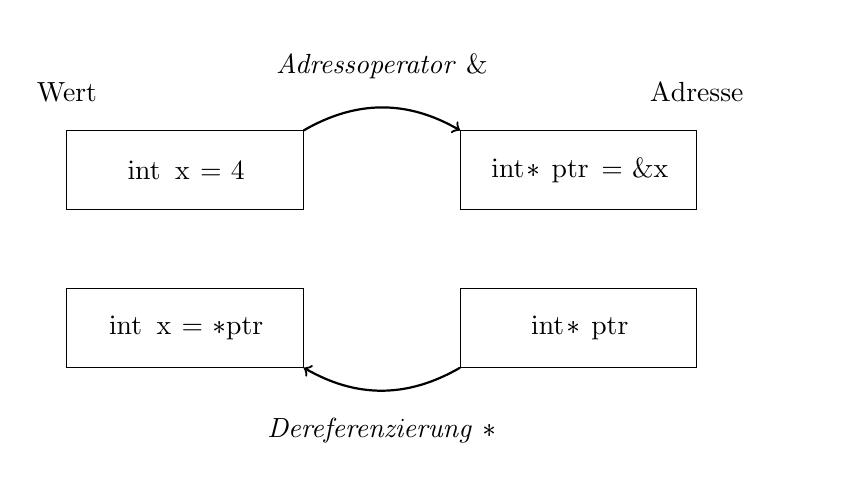
\begin{tikzpicture}[every node/.style={draw, minimum height=1cm, minimum width=3cm}]
		
		\node[rectangle] (wert) at (0,0) {\lstinline|int x = 4|};
		\node[rectangle] (adr) at (5,0) {\lstinline|int* ptr = &x|};
		\path[->, draw, thick] (wert.north east) to[bend left] node[above, draw=none] {\textit{Adressoperator} \lstinline|&|} (adr.north west);
		
		\node[rectangle] (wert2) at (0,-2) {\lstinline|int x = *ptr|};
		\node[rectangle] (adr2) at (5,-2) {\lstinline|int* ptr|};
		\path[->, draw, thick] (adr2.south west) to[bend left] node[below, draw=none] {\textit{Dereferenzierung} \lstinline|*|} (wert2.south east);
		
		\node[draw=none, minimum height=0, minimum width=0] at (-1.5,1) {Wert};
		\node[draw=none] at(6.5,1) {Adresse};
		\end{tikzpicture}}
	\end{center}

	\textbf{Nutzen}: \enquote{Verlängerung} Sichtbarkeit von Variablen (Veränderung innerhalb von Funktionen \enquote{speichern}), dynamische Datentypen
\end{frame}

\begin{frame} \frametitle{Array-Pointer-Dualität}	
	\small
	Ein Array ist ein Pointer, der auf die erste Komponente des Arrays zeigt.
	\begin{center}
		\scalebox{0.8}{
			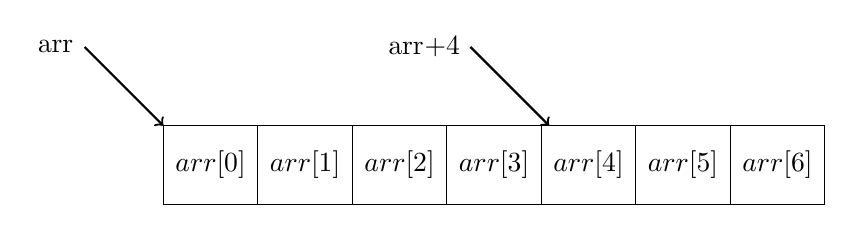
\begin{tikzpicture}%[every node/.style={draw, minimum height=1cm, minimum width=3cm}]
			
				
			
			\foreach \i in {0,...,6} {
				\draw[] (\i*1.2,-1) rectangle ++(1.2,1) node[pos=.5] (arr\i) {$arr[\i]$};
			}	
			\path[->, draw, thick] (-1,1) to node[pos=0, left]{\lstinline|arr|} (0,0);
			\path[->, draw, thick] (4*1.2-0.9,1) to node[pos=0, left]{\lstinline|arr+4|} (4*1.2 + 0.1,0);	
			\end{tikzpicture}}
	\end{center}
	
	\textbf{Pointerarithmetik}: \lstinline|ptr + i| zeigt auf die \lstinline|i|-te Speicherzelle nach \lstinline|ptr| (analog \lstinline|ptr - i|, \lstinline|ptr++| usw.)
	
	Der Elementzugriff \lstinline|arr[i]| ist gleichbedeutend mit \lstinline|*(arr + i)|.
\end{frame}

\begin{frame}[fragile] \frametitle{Aufgabe 1}
	\begin{lstlisting}[basicstyle=\ttfamilywithbold\scriptsize]
void palindrom(char str[], int l, int *korrekt) {
	int i = 0;
	l = l - 1;
	*korrekt = 1;
	
	while (i < l && *korrekt) {
		*korrekt = str[i] == str[l];
		i = i + 1;
		l = l - 1;
	}
}

int main () {
	char[...] str;
	int korr;
	int len;
	...
	palindrom(str, len, &korr);
}
	\end{lstlisting}
\end{frame}

%%%%%%%%%%%%%%%%%%%%%%%%%%%%%%%%%%%%%%%%%%%%%%%%%%%%%%%%%%%%%%%%%%%%%%%%%%%%%%%%%%%
\begin{frame} \frametitle{Aufgabe 2}
	\centering
	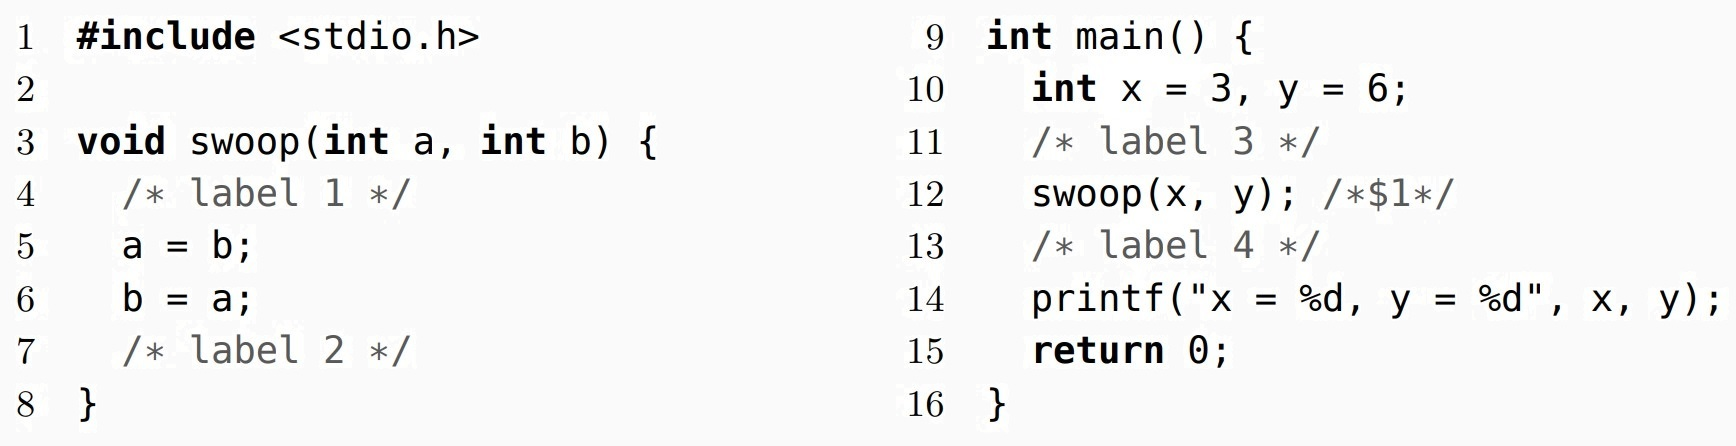
\includegraphics[width=\textwidth]{./tut05_aufgabe2.jpg}
\end{frame}

\begin{frame} \frametitle{Aufgabe 2 --- Teil (a)}
	\centering
	\def\arraystretch{0.9}
	\begin{tabular}{|p{1.5cm}|r||R{0.4cm}|R{0.4cm}|R{0.4cm}|R{0.4cm}|}
		\hline
		Label & RM & 1 & 2 & 3 & 4 \\ 
		\hline \hline
		\multirow{2}{*}{label3} & \multirow{2}{*}{---} & x & y &   & \\ 
		&                      & 3 & 6 &   & \\ \hline
		\multirow{2}{*}{label1} & \multirow{2}{*}{1}   &   &   & a & b \\      
		&                      &   &   & 3 & 6 \\ \hline
		\multirow{2}{*}{label2} & \multirow{2}{*}{1}   &   &   & a & b \\    
		&                      &   &   & 6 & 6 \\ \hline  
		\multirow{2}{*}{label4} & \multirow{2}{*}{---} & x & y &   &   \\ 
		&                      & 3 & 6 &   &   \\ \hline
	\end{tabular}
\end{frame}

\begin{frame}[fragile] \frametitle{Aufgabe 2 --- Teil (b)}
\begin{lstlisting}
#include <stdio.h>
void swap(int *a, int *a){ 
	int tmp;
	tmp = *a; 
	*a = *b;
	*b = tmp;
}
int main() {
	int x = 4, y = 6;
	printf("x = %d, y = %d \n", x, y);
	swap(&x, &y);
	printf("x = %d, y = %d \n", x, y);
	return 0;
}
\end{lstlisting}
\end{frame}

%%%%%%%%%%%%%%%%%%%%%%%%%%%%%%%%%%%%%%%%%%%%%%%%%%%%%%%%%%%%%%%%%%%%%%%%%%%%%%%%%%%

\begin{frame} \frametitle{Pulsierender Speicher}
	\small
	\textbf{Gültigkeitsbereiche von Objekten}:
	\begin{itemize}
		\item Eine Funktion ist ab ihrer Deklaration bis zum Programmende sichtbar. Vorwärtsdeklarationen beachten!
		\item  Ihre formalen Parameter jedoch nur innerhalb der Funktionsdefinition!
		\item Gibt es gleichlautende formale Parameter in verschiedenen Funktionen, müssen diese in der Tabelle natürlich unterschieden werden (z.B. durch \enquote{x in f}).
		\item Vorsicht bei Namenskonflikten: lokale Variablen überschreiben die Sichtbarkeit globaler Variablen.
	\end{itemize}
\end{frame}

\begin{frame} \frametitle{Pulsierender Speicher}
	\small
	\textbf{Speicherprotokoll}:
	\begin{itemize}
		\item Für jeden Funktionsaufruf werden erst die Parameter, dann die lokalen Variablen in Reihenfolge ihres Auftretens in der Umgebung notiert. Globale Variablen stehen ganz vorn.
		\item Variablennamen werden nur notiert, wenn die Variablen sichtbar sind. Globale Variablennamen werden immer notiert.
		\item Der Wert von nicht sichtbaren Variablen muss nur notiert werden wenn er sich ändert.
		\item Uninitialisierte Variablen werden mit Inhalt \enquote{?} notiert.
	\end{itemize}
\end{frame}

\begin{frame} \frametitle{Aufgabe 3}
	\centering
	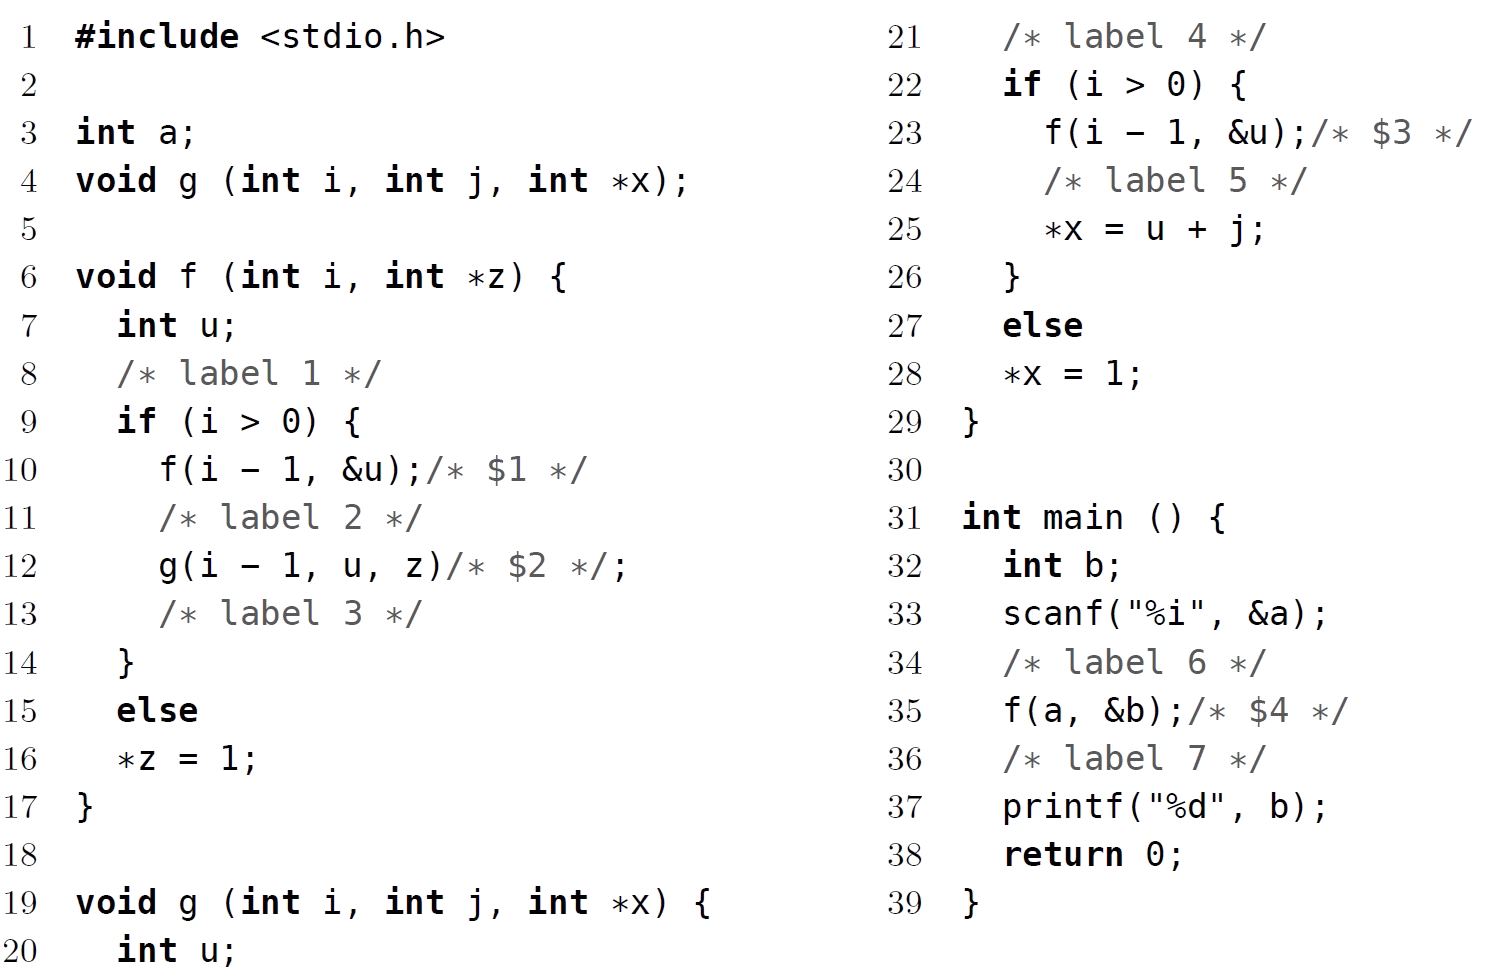
\includegraphics[width=\textwidth]{./tut05_aufgabe3.png}
\end{frame}

\begin{frame} \frametitle{Aufgabe 3 --- Teil (a)}
	\textbf{Gültigkeitsbereiche}

	\centering
	\begin{tabular}{|l|c|}
		\hline
		Objektname & Gültigkeitsbereich \\ \hline \hline
		\texttt{a} & 2 -- 14 und 25 -- 33 \\ \hline
		\texttt{g} & 4 -- 33 \\ \hline
		\texttt{a, b} in \texttt{g} & 15 -- 24 \\ \hline
		\texttt{i} in \texttt{g} & 16 -- 24 \\ \hline
		\texttt{f} & 6 -- 33 \\ \hline
		\texttt{i,j} in \texttt{f} & 6 -- 13 \\ \hline
		\texttt{main} & 26 -- 33 \\ \hline
		\texttt{x} in \texttt{main} & 27 -- 33 \\ \hline
	\end{tabular}
\end{frame}


\begin{frame} \frametitle{Aufgabe 3 --- Teil (b)}
	\centering
	\scalebox{0.6}{
	\def\arraystretch{0.9}
	\begin{tabular}{|p{1cm}|r||R{0.25cm}||R{0.25cm}|R{0.25cm}|R{0.25cm}|R{0.25cm}|R{0.25cm}|R{0.25cm}|R{0.25cm}|R{0.25cm}|R{0.25cm}|R{0.25cm}|R{0.25cm}|}
		\hline
		Label & RM & 1 & 2 & 3 & 4 & 5 & 6 & 7 & 8 & 9 & 10 & 11 & 12 \\ 
		\hline \hline
		label5 & --      & a & x &   &   &   &   &   &   &   &   &   & \\ 
	           &         & 7 & 0 &   &   &   &   &   &   &   &   &   & \\ \hline
		label3 & 3       &   &   & a & b & i &   &   &   &   &   &   & \\ 
		       &         &   &   & 7 & 2 & 2 &   &   &   &   &   &   & \\ \hline
		label1 & 2:3     & a &   &   &   &   & i & j &   &   &   &   & \\ 
		       &         & 7 &   &   &   &   & 5 & 7 &   &   &   &   & \\ \hline
		label2 & 2:3     & a &   &   &   &   & i & j &   &   &   &   & \\ 
			   &         & 7 &   &   &   &   & 5 & 7 &   &   &   &   & \\ \hline
		label4 & 3       &   &   & a & b & i &   &   &   &   &   &   & \\ 
			   &         &   & 1 & 3 & 2 & 2 &   &   &   &   &   &   & \\ \hline
		label1 & 2:3     & a &   &   &   &   & i & j &   &   &   &   & \\ 
		       &         & 7 &   &   &   &   & 5 & 3 &   &   &   &   & \\ \hline
		label1 & 1:2:3   & a &   &   &   &   &   &   & i & j &   &   & \\ 
			   &         & 7 &   &   &   & 3 &   &   & 5 & 3 &   &   & \\ \hline
		label1 & 1:1:2:3 & a &   &   &   &   &   &   &   &   & i & j & \\ 
			   &         & 7 &   &   &   & 4 &   &   &   &   & 5 & 3 & \\ \hline
		label2 & 1:1:2:3 & a &   &   &   &   &   &   &   &   & i & j & \\ 
			   &         & 7 &   &   &   &   &   &   &   &   & 5 & 3 & \\ \hline
		label2 & 1:2:3   & a &   &   &   &   &   &   & i & j &   &   & \\ 
		       &         & 7 &   &   &   &   &   &   & 5 & 3 &   &   & \\ \hline
		label2 & 2:3     & a &   &   &   &   & i & j &   &   &   &   & \\ 
		       &         & 7 &   &   &   &   & 5 & 3 &   &   &   &   & \\ \hline
		label4 & 3       &   &   & a & b & i &   &   &   &   &   &   & \\ 
			   &         &   & 2 & 1 & 2 & 4 &   &   &   &   &   &   & \\ \hline
		label6 & --      & a & x &   &   &   &   &   &   &   &   &   & \\ 
			   &         & 7 & 2 &   &   &   &   &   &   &   &   &   & \\ \hline
	\end{tabular}}
\end{frame}



%%%%%%%%%%%%%%%%%%%%%%%%%%%%%%%%%%%%%%%%%%%%%%%%%%%%%%%%%%%%%%%%%%%%%%%%%%%%%%%%%%%

\end{document}